\chapterimage{orange2.jpg} % Chapter heading image
\chapterspaceabove{6.75cm} % Whitespace from the top of the page to the chapter title on chapter pages
\chapterspacebelow{7.25cm} % Amount of vertical whitespace from the top margin to the start of the text on chapter pages

\chapter{Passivity}\index{Passivity}
\section{Overview}\index{Overview}
This chapter introduces \emph{passivity theory} as a framework for analyzing the stability of feedback systems. 
Our focus is on the \textbf{input--output definition} of passivity, with the goal of establishing 
\textbf{open-loop conditions} that guarantee \textbf{closed-loop stability}. 
The passivity approach provides an intuitive, energy-based viewpoint, in close parallel with the 
\textbf{small gain theorem}.

\section{Power and Energy: Passive Systems}\index{Power and Energy: Passive Systems}

Before introducing passivity for abstract dynamical systems, it is helpful to recall 
simple examples from circuit theory. From physics, the instantaneous \emph{power} $p(t)$ 
absorbed by a device is defined as the rate of change of its stored energy $w(t)$:
\begin{equation}
    p(t) = \frac{d w(t)}{dt},
\end{equation}
where the total energy absorbed up to time $t$ is
\begin{equation}
    w(t) = \int_{0}^{t} p(\tau)\, d\tau.
\end{equation}

\subsection{Example: A Circuit Element}

\begin{figure}[h]
    \centering
    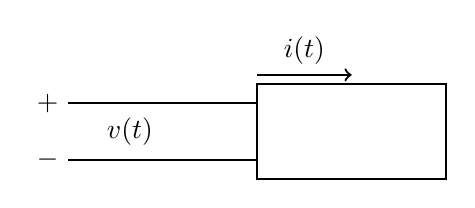
\begin{tikzpicture}[scale=1.2]
        % Box
        \draw[thick] (2,0.5) rectangle (4,-0.5);
        % Voltage source terminals
        \draw[thick] (0,0.3) -- (2,0.3);
        \draw[thick] (0,-0.3) -- (2,-0.3);
        % Labels
        \node[left] at (0,0.3) {$+$};
        \node[left] at (0,-0.3) {$-$};
        % Current arrow
        \draw[->,thick] (2,0.6) -- (3,0.6) node[midway,above] {$i(t)$};
        % Voltage label
        \node[left] at (1,0) {$v(t)$};
    \end{tikzpicture}
    \caption{A two-terminal circuit element.}
    \label{fig:passive_element}
\end{figure}

For such an element, with terminal voltage $v(t)$ and current $i(t)$ entering the box, 
the instantaneous power is
\begin{equation}
    p(t) = v(t)\, i(t).
\end{equation}
Accordingly, the energy absorbed up to time $t$ is
\begin{equation}
    w(t) = \int_{0}^{t} v(\tau) i(\tau)\, d\tau.
\end{equation}

\noindent Two cases can occur:
\begin{itemize}
    \item $w(t) > 0$: the device \emph{absorbs} energy (e.g., a resistor).
    \item $w(t) < 0$: the device \emph{delivers} energy (e.g., an ideal battery).
\end{itemize}

\begin{definition}[Passive Element]
A device is said to be \emph{passive} if it never generates its own energy, i.e.,
\begin{equation}
    \int_{-\infty}^{t} v(\tau) i(\tau)\, d\tau \;\geq\; 0,
    \qquad \forall t.
\end{equation}
\end{definition}

\subsection{Example: A Passive Network Driven by a Source}

\begin{figure}[h!]
    \centering
    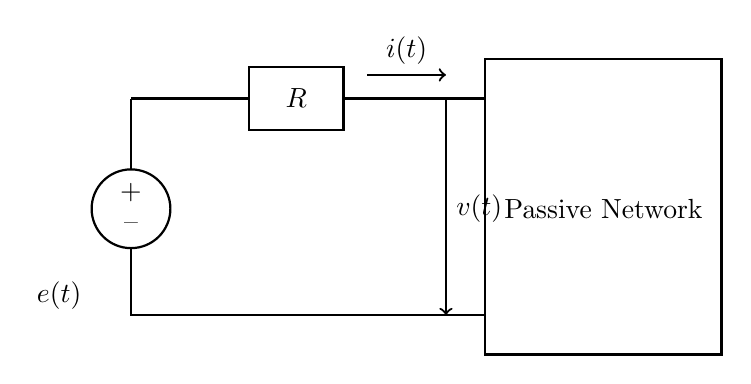
\begin{tikzpicture}[thick]
        % Voltage source
        \draw (0,1.1) circle (0.5);
        \node at (0,1.3) {+};
        \node at (0,0.9) {--};
        \node[left] at (-0.5,0) {$e(t)$};

        % Terminals
        \draw (0,1.6)-- (0,2.5);
        \draw (0,0.6) |- (1.5,-0.25);

        % Upper wire
        \draw (0,2.5) -- (1.5,2.5);

        % Resistor
        \draw (1.5,2.1) rectangle (2.7,2.9);
        \node at (2.1,2.5) {$R$};

        % Wires to passive block
        \draw (2.7,2.5) -- (4.5,2.5);
        \draw (1.5,-0.25) -- (4.5,-0.25);

        % Passive block
        \draw (4.5,-0.75) rectangle (7.5,3);
        \node at (6,1.1) {Passive Network};

        % Labels
        \draw[<-] (4,-0.25) -- (4,2.5);
        \node[right] at (4,1.1) {$v(t)$};
        \draw[->] (3.0,2.8) -- (4.0,2.8) node[midway,above] {$i(t)$};
    \end{tikzpicture}
    \caption{A passive network driven by a source.}
    \label{fig:passive_network}
\end{figure}

Applying Kirchhoff’s voltage law,
\begin{equation}
    e(t) = R i(t) + v(t).
\end{equation}
If the source $e(t)$ is square integrable,
\begin{equation}
    \int_{0}^{\infty} e^{2}(t)\, dt < \infty,
\end{equation}
then both $i(t)$ and $v(t)$ also have finite energy. In other words, the passive network 
cannot produce unbounded signals on its own and is therefore \emph{well behaved}. 

\medskip
\noindent More generally, the total absorbed energy can be decomposed as
\begin{equation}
    w(t) = \underbrace{\int_{0}^{t} v(\tau) i(\tau)\, d\tau}_{\text{input-dependent}}
          + \underbrace{\int_{-\infty}^{0} v(\tau) i(\tau)\, d\tau}_{\text{initial conditions}}.
\end{equation}
The first term accounts for the effect of the applied input after $t=0$, 
while the second captures the contribution of nonzero initial conditions.  

With the sign convention of Fig.~\ref{fig:passive_element}, passivity requires
\begin{equation}
    \int_{-\infty}^{t} v(\tau) i(\tau)\, d\tau \;\geq\; 0, \qquad \forall t,
\end{equation}
which holds for resistors, capacitors, and inductors. 
Thus these are classified as \emph{passive elements}, and more generally, 
passive networks behave in a controlled, non-energy-generating manner.

\section{Definitions}\index{Definitions}

To formalize the concept of passivity we require some basic tools from functional analysis,
in particular the notion of an inner product space.

\begin{definition}[Inner Product Space]
A \emph{real inner product space} is a real vector space $X$ equipped with a mapping
\begin{equation}
    \langle \cdot, \cdot \rangle : X \times X \to \mathbb{R},
\end{equation}
called an \emph{inner product}, such that for all $x,y,z \in X$ and $\alpha \in \mathbb{R}$:
\begin{enumerate}
    \item Symmetry:
    \begin{equation}
        \langle x, y \rangle = \langle y, x \rangle,
    \end{equation}
    \item Linearity in the first argument:
    \begin{equation}
        \langle x+y, z \rangle = \langle x,z \rangle + \langle y,z \rangle,
    \end{equation}
    \begin{equation}
        \langle \alpha x, y \rangle = \alpha \langle x,y \rangle,
    \end{equation}
    \item Positive-definiteness:
    \begin{equation}
        \langle x,x \rangle \ge 0, 
        \qquad \langle x,x \rangle = 0 \;\; \Leftrightarrow \;\; x=0.
    \end{equation}
\end{enumerate}
The norm induced by the inner product is
\begin{equation}
    \|x\| = \sqrt{\langle x,x \rangle}.
\end{equation}
If $X$ is complete with respect to this norm, then $X$ is called a \emph{Hilbert space}.
\end{definition}

\begin{example}[Euclidean Space]
Let $X = \mathbb{R}^n$. The standard dot product
\begin{equation}
    \langle x,y \rangle = x^\top y = x_1 y_1 + x_2 y_2 + \cdots + x_n y_n
\end{equation}
defines an inner product, making $\mathbb{R}^n$ an inner product space.
\end{example}

\begin{remark}[\textbf{Cauchy--Schwarz Inequality}]
For any $x,y \in X$,
\begin{equation}
    |\langle x, y \rangle| \le \|x\|\, \|y\|.
\end{equation}
\end{remark}

\medskip
\noindent
In the study of dynamical systems, we often take $X$ to be a function space such as 
$L^2[0,\infty)$ with the natural inner product
\begin{equation}
    \langle x, y \rangle = \int_{0}^{\infty} x(t)\, y(t)\, dt.
\end{equation}

\begin{definition}[Passive System]
A system $H : X_e \to X_e$ is called \emph{passive} if
\begin{equation}
    \langle u, Hu \rangle_T \;\geq\; \beta,
    \qquad \forall u \in X_e, \; \forall T \ge 0,
\end{equation}
where $\langle \cdot, \cdot \rangle_T$ denotes the inner product truncated at time $T$ and 
$\beta$ accounts for energy that may have been stored at $t=0$.
\end{definition}

\begin{definition}[Strictly Passive System]
A system $H : X_e \to X_e$ is \emph{strictly passive} if there exists $\delta > 0$ such that
\begin{equation}
    \langle u, Hu \rangle_T \;\geq\; \delta \|u\|_T^2 + \beta,
    \qquad \forall u \in X_e, \; \forall T \ge 0.
\end{equation}
Here $\|u\|_T$ denotes the truncated norm on $[0,T]$, and $\beta$ again represents possible
initial stored energy.
\end{definition}

\begin{example}[Network Example]
Consider the network of Figure~\ref{fig:passive_element} with input $u = v(t)$ (voltage)
and output $y = Hu = i(t)$ (current). The passivity condition reads
\begin{equation}
    \langle v, i \rangle_T 
    = \int_{0}^{T} v(t)\, i(t)\, dt \;\geq\; 0,
    \qquad \forall T \ge 0,
\end{equation}
which is exactly the statement that the network cannot generate energy on its own.
\end{example}

\begin{definition}[Positive and Strictly Positive Systems]
A system $H : X \to X$ is \emph{positive} if
\begin{equation}
    \langle u, Hu \rangle \;\geq\; \beta, 
    \qquad \forall u \in X.
\end{equation}
It is \emph{strictly positive} if there exists $\delta > 0$ such that
\begin{equation}
    \langle u, Hu \rangle \;\geq\; \delta \|u\|^2 + \beta, 
    \qquad \forall u \in X.
\end{equation}
\end{definition}

\begin{theorem}[Equivalence of Passivity and Positivity]
Let $H : X \to X$ be a causal system. Then:
\begin{enumerate}
    \item $H$ is positive $\;\Leftrightarrow\;$ $H$ is passive.
    \item $H$ is strictly positive $\;\Leftrightarrow\;$ $H$ is strictly passive.
\end{enumerate}
\end{theorem}

\medskip
\noindent
Thus, under causality and stability assumptions, the notions of passivity and positivity
coincide. This equivalence will be useful in establishing stability properties of 
feedback interconnections.

\section{Interconnections of Passive Systems}\index{Interconnections of Passive Systems}

In many situations it is important to analyze how passivity properties are preserved
when subsystems are interconnected. Two particularly relevant cases are \emph{parallel
interconnections} and \emph{feedback interconnections}. 

% Figure 1: Parallel sum H1 + H2 + ... + Hn
\begin{figure}[!h]
\centering
\begin{tikzpicture}[>=Stealth, node distance=1.2cm, every node/.style={font=\Large}]
    % Blocks
    \node[draw, minimum width=2cm, minimum height=1cm] (H1) at (0,0) {H1};
    \node[draw, minimum width=2cm, minimum height=1cm, above=1cm of H1] (H2) {H2};
    \node[draw, minimum width=2cm, minimum height=1cm, above=1cm of H2] (Hn) {Hn};

    % Input
    \node[left=3cm of H1] (u) {$u(t)$};
    
    % Arrows from input to blocks
    \draw[->] (u.east) -- (H1.west);
    \draw[->] (u.east) -- ++(0,2) -- (H2.west);
    \draw[->] (u.east) -- ++(0,4) -- (Hn.west);

    % Summing junction
    \node[circle, draw, minimum size=0.35cm, right=3cm of H1] (sum) {};
    
    % Arrows from blocks to summing junction
    \draw[->] (H1.east) -- (sum.west);
    \draw[->] (H2.east) -- ++(3,0) |- (sum.north);
    \draw[->] (Hn.east) -- ++(3,0) |- (sum.north);

    % Output
    \node[right=2cm of sum] (y) {$y(t)$};
    \draw[->] (sum.east) -- (y.west);
\end{tikzpicture}
\caption{Parallel interconnection $H = H_1 + H_2 + \cdots + H_n$.}
\label{fig:parallel_sum}
\end{figure}

% Figure 2: Feedback system S1
\begin{figure}[!h]
\centering
\begin{tikzpicture}[>=Stealth, node distance=1.5cm, every node/.style={font=\Large}]
    % Summing junction
    \node[circle, draw, minimum size=0.35cm] (sum) {};
    \node[left=2cm of sum] (u) {$u(t)$};
    \draw[->] (u.east) -- (sum.west);
    \node[above left=0.2cm and 0.2cm of sum] {$+$};
    \node[below left=0.2cm and 0.2cm of sum] {$-$};

    % Forward path blocks
    \node[draw, minimum width=2cm, minimum height=1cm, right=2cm of sum] (H1) {H1};
    \node[draw, minimum width=2cm, minimum height=1cm, below=2cm of H1] (H2) {H2};

    % Forward arrows
    \node[right=2cm of H1] (y) {$y(t)$};
    \draw[->] (sum.east) -- (H1.west) node[midway, above] {$e_1(t)$};
    \draw[->] (H1.east) -- (y.west);

    % Feedback path
    \draw[->] (y.south) |- (H2.east);
    \draw[->] (H2.west) -| (sum.south) node[pos=0.25, above] {$y_2(t)$};
\end{tikzpicture}
\caption{Feedback interconnection of $H_1$ and $H_2$.}
\label{fig:feedback_system}
\end{figure}

\begin{theorem}[Interconnection of Passive Systems]\index{Interconnection of Passive Systems}
Consider a finite number of systems $H_i : X_e \to X_e$, $i = 1, \dots, n$.
\begin{enumerate}
    \item \textbf{Parallel interconnection:}  
    If all the systems $H_i$ are passive, then
    \begin{equation}\label{eq:parallel}
        H = H_1 + H_2 + \cdots + H_n
    \end{equation}
    (see Figure~\ref{fig:parallel_sum}) is passive.
    
    \item \textbf{Strict passivity:}  
    If all the systems $H_i$ are passive, and at least one of them is strictly passive, then
    the system $H$ in \eqref{eq:parallel} is strictly passive.
    
    \item \textbf{Feedback interconnection:}  
    If $H_1$ and $H_2$ are passive and the feedback interconnection
    \begin{align}
        e(t) &= u(t) - H_2 y(t), \label{eq:feedback1}\\
        y(t) &= H_1 e(t), \label{eq:feedback2}
    \end{align}
    (see Figure~\ref{fig:feedback_system}) is well-defined (i.e., $e(t) \in X_e$ is uniquely
    determined for each $u(t) \in X_e$), then the overall mapping from $u$ to $y$ is passive.
\end{enumerate}
\end{theorem}

\begin{remark}
The results in parts (1) and (2) do not automatically extend to an infinite number of systems.  
Such extensions depend on the properties of the inner product space. In particular, 
if the inner product is the standard one in $L^2$, then the extension to infinite sums is valid.
\end{remark}

\subsection{Passivity and Small Gain}\index{Interconnection of Passive Systems!Passivity and Small Gain}

The concept of passivity is closely related to the \emph{small gain condition}. 
Given an inner product space $X_e$, define the induced gain of a system 
$H: X_e \to X_e$ by the norm
\begin{equation}
    \|x\|^2 = \langle x, x \rangle.
\end{equation}

\begin{theorem}[Passivity and Small Gain]\index{Passivity and Small Gain}
Let $H: X_e \to X_e$ and assume that $(I + H)$ is invertible on $X_e$, i.e.,
\begin{equation}
    (I + H)^{-1}: X_e \to X_e.
\end{equation}
Define
\begin{equation}
    S = (H - I)(I + H)^{-1}.
\end{equation}
Then:
\begin{enumerate}
    \item $H$ is passive $\;\Leftrightarrow\;$ the gain of $S$ is at most $1$, i.e.,
    \begin{equation}
        \|Sx\|_T \le \|x\|_T, 
        \qquad \forall x \in X_e, \; \forall T \ge 0.
    \end{equation}
    \item $H$ is strictly passive with finite gain $\;\Leftrightarrow\;$ the gain of $S$ is strictly less than $1$.
\end{enumerate}
\end{theorem}

\section{Stability of Feedback Interconnections}\index{Stability of Feedback Interconnections}

Feedback interconnections of passive systems play an important role in stability 
analysis. Consider two systems $H_1, H_2 : X_e \to X_e$ interconnected in feedback 
(see Figure~\ref{fig:feedback_system}) according to
\begin{align}
    e_1(t) &= u_1(t) - H_2 e_2(t), \label{eq:stab_feedback1}\\
    y_1(t) &= H_1 e_1(t). \label{eq:stab_feedback2}
\end{align}

\begin{theorem}[Passivity-Based Stability, Single Input]\label{thm:passivity1}
If $H_1$ is passive and $H_2$ is strictly passive, then for any $u_1 \in X$, 
the output $y_1 \in X$.  
In other words, the closed-loop system is input-output stable.
\end{theorem}

\begin{remark}
Theorem~\ref{thm:passivity1} guarantees boundedness of $y_1$ for bounded input $u_1$, 
but does not ensure that the internal signals $e_1$ or $y_2$ are bounded.  
A stronger condition—strict passivity with finite gain—is required to bound all signals.
\end{remark}

\begin{theorem}[Passivity-Based Stability with Finite Gain]\label{thm:passivity2}
If $H_1$ and $H_2$ are passive, and one of them is strictly passive with finite gain, 
then all internal signals $e_1, e_2$ and outputs $y_1, y_2$ belong to $X$ 
for any $u_1 \in X$.
\end{theorem}

\begin{remark}
This theorem strengthens Theorem~\ref{thm:passivity1} by ensuring closed-loop 
boundedness of \emph{all} signals in the interconnection, not only the external outputs.
\end{remark}

\begin{figure}[!ht]
\centering
\resizebox{0.9\textwidth}{!}{%
\begin{tikzpicture}
\tikzstyle{every node}=[font=\normalsize]

% Nodes
\draw  (4.25,13.75) circle (0.25cm);
\draw  (9.25,11.25) circle (0.25cm);
\draw  (5.75,14.25) rectangle (7.75,13.25);
\draw  (5.75,11.75) rectangle (7.75,10.75);

% Arrows
\draw [->, >=Stealth] (4.5,13.75) -- (5.75,13.75);
\draw [->, >=Stealth] (9,11.25) -- (7.75,11.25);
\draw [->, >=Stealth] (7.75,13.75) -- (10,13.75);
\draw [short] (5.75,11.25) -- (4.25,11.25);
\draw [->, >=Stealth] (4.25,11.25) -- (4.25,13.5);
\draw [->, >=Stealth] (9.25,13.75) -- (9.25,11.5);
\draw [->, >=Stealth] (3,13.75) -- (4,13.75);
\draw [->, >=Stealth] (10,11.25) -- (9.5,11.25);

% Labels
\node [font=\normalsize] at (6.75,13.75) {H1};
\node [font=\normalsize] at (6.75,11.25) {H2};
\node [font=\normalsize] at (10.5,13.75) {$y_1(t)$};
\node [font=\normalsize] at (5,11.5) {$y_2(t)$};
\node [font=\normalsize] at (2.5,13.75) {$u_1(t)$};
\node [font=\normalsize] at (10.5,11.25) {$u_2(t)$};
\node [font=\normalsize] at (5,14) {$e_1(t)$};
\node [font=\normalsize] at (8.5,11.5) {$e_2(t)$};
\end{tikzpicture}
}%
\caption{Two-input feedback interconnection.}
\label{fig:feedback_two}
\end{figure}

\begin{theorem}[Two-Input Feedback System]\label{thm:passivity3}
Consider the two-input feedback system of Figure~\ref{fig:feedback_two}, defined by
\begin{align}
    e_1(t) &= u_1(t) - H_2 e_2(t), \label{eq:twoinput1}\\
    e_2(t) &= u_2(t) + H_1 e_1(t). \label{eq:twoinput2}
\end{align}
If both $H_1$ and $H_2$ are passive, and at least one of them is strictly passive 
with finite gain, then all signals $e_1, e_2, y_1, y_2$ belong to $X$ 
for any $u_1, u_2 \in X$.
\end{theorem}

\begin{remark}
Theorems~\ref{thm:passivity2} and \ref{thm:passivity3} provide the foundation for 
passivity-based stability analysis.  
They ensure input-output stability of feedback interconnections under mild and 
physically interpretable conditions.
\end{remark}

\section{Passivity of LTI Systems}\index{Passivity of LTI Systems}

We now turn to the implications of passivity in the important case of 
linear time-invariant (LTI) systems. Throughout this section, signals are assumed 
to belong to the energy space $L_2$, and we work primarily in the frequency domain 
using Fourier transforms.  

\subsection{SISO Case}

For single-input single-output systems, the passivity property is conveniently 
characterized in terms of the real part of the frequency response.  

\begin{theorem}[Passivity of SISO LTI Systems]\label{thm:siso_passivity}
Let $H : L_{2e} \to L_{2e}$ be an LTI operator defined by convolution
\begin{equation}
Hx = h * x, 
\qquad h \in \mathcal{A},\; x \in L_{2e}.
\end{equation}
Then:
\begin{enumerate}
    \item $H$ is \textbf{passive} if and only if
    \begin{equation}
    \Re\!\left\{H(j\omega)\right\} \ge 0,
    \qquad \forall \omega \in \mathbb{R}.
    \end{equation}
    \item $H$ is \textbf{strictly passive} if and only if there exists $\beta>0$ such that
    \begin{equation}
    \Re\!\left\{H(j\omega)\right\} \ge \beta,
    \qquad \forall \omega \in \mathbb{R}.
    \end{equation}
\end{enumerate}
\end{theorem}

\begin{remark}
The proof follows directly from Parseval’s relation. Passivity corresponds to 
nonnegative energy dissipation at each frequency, while strict passivity requires a 
uniform positive margin $\beta$, ensuring that the system always dissipates energy. 
\end{remark}

\subsection{MIMO Case}

For multi-input multi-output systems, the passivity condition is expressed in terms 
of the Hermitian part of the transfer matrix.  

\begin{theorem}[Passivity of MIMO LTI Systems]\label{thm:mimo_passivity}
Let $H : L_{2e} \to L_{2e}$ be an LTI operator with transfer matrix $H(j\omega)$. Then:
\begin{enumerate}
    \item $H$ is \textbf{passive} if and only if
    \begin{equation}
    H(j\omega) + H(j\omega)^* \;\succeq\; 0, 
    \qquad \forall \omega \in \mathbb{R}.
    \end{equation}
    \item $H$ is \textbf{strictly passive} if and only if there exists $\beta > 0$ such that
    \begin{equation}
    \lambda_{\min}\!\left( H(j\omega) + H(j\omega)^* \right) \ge \beta,
    \qquad \forall \omega \in \mathbb{R},
    \end{equation}
    where $\lambda_{\min}$ denotes the minimum eigenvalue.
\end{enumerate}
\end{theorem}

\begin{remark}
The matrix inequality in Theorem~\ref{thm:mimo_passivity} states that the Hermitian part 
of $H(j\omega)$ is positive semidefinite for all frequencies. This generalizes the SISO 
condition $\Re\{H(j\omega)\} \ge 0$.  
\end{remark}

\subsection{Example: Oscillatory First-Order Systems}

As an illustration, consider the transfer function
\begin{equation}
H(s) = \frac{\alpha s}{s^2 + \omega_0^2},
\qquad \alpha > 0, \;\; \omega_0 > 0.
\end{equation}

\begin{theorem}[Passivity of Oscillatory First-Order Systems]\label{thm:oscillatory_passivity}
The system with transfer function $H(s) = \tfrac{\alpha s}{s^2 + \omega_0^2}$ is 
\textbf{passive}.
\end{theorem}

\begin{remark}
Indeed, evaluating along the imaginary axis shows $\Re\{H(j\omega)\} \ge 0$ for all 
$\omega$. The system does not generate energy and is often used to model oscillatory 
modes in flexible structures.  
\end{remark}

\section{Strictly Positive Real Rational Functions}\index{Strictly Positive Real Rational Functions}

The condition for strict passivity derived above,
\begin{equation}
\Re\{H(j\omega)\} \ge \beta > 0, \qquad \forall \omega,
\end{equation}
is generally too strong: no strictly proper rational system can satisfy it.  
To overcome this limitation, we turn to the notion of 
\emph{strictly positive real (SPR)} functions, which provide a weaker yet useful 
requirement for stability analysis.  

\begin{definition}[Positive Real (PR) and Strictly Positive Real (SPR)]
A rational function $H(s) = \tfrac{p(s)}{q(s)}$ is:
\begin{itemize}
    \item \textbf{Positive real (PR)} if $\Re\{H(s)\} \ge 0$ for all $s$ with $\Re[s] > 0$.
    \item \textbf{Strictly positive real (SPR)} if there exists $\epsilon > 0$ such that 
    $H(s-\epsilon)$ is PR.
\end{itemize}
\end{definition}

\begin{definition}[Class $\mathcal{Q}$ and Weak SPR]
A rational function $H(s) = p(s)/q(s)$ belongs to class $\mathcal{Q}$ if:
\begin{enumerate}
    \item $q(s)$ is \emph{Hurwitz}, i.e., all roots of $q(s)$ lie strictly in the open 
    left-half complex plane ($\Re[s] < 0$),
    \item $\Re\{H(j\omega)\} > 0$ for all $\omega \ge 0$.
\end{enumerate}
It is called \textbf{weak SPR} if it is in class $\mathcal{Q}$ and satisfies
$\deg(p) - \deg(q) \le 1$.  
It is called \textbf{SPR} if it is weak SPR and in addition:
\begin{enumerate}
    \item $\deg(p) = \deg(q)$, or
    \item $\deg(p) = \deg(q)+1$ with $\lim_{\omega\to\infty} \Re\{H(j\omega)\} > 0$.
\end{enumerate}
\end{definition}

\begin{corollary}[Kalman--Yakubovich]
Consider the state-space system
\begin{equation}
\dot{x} = Ax + Bu, 
\qquad y = Cx + Du,
\end{equation}
with $x \in \mathbb{R}^n$, $u \in \mathbb{R}^m$, $y \in \mathbb{R}^m$.  
Assume $A$ is Hurwitz, $(A,B)$ controllable, and $(C,A)$ observable.  
Then the transfer function 
\begin{equation}
H(s) = C(sI-A)^{-1}B + D
\end{equation}
is SPR if and only if there exist $P = P^\top \succ 0$, and matrices $Q,W$, together 
with sufficiently small $\epsilon > 0$, such that
\begin{align}
PA + A^\top P &= -QQ^\top - \epsilon P, \\
PB + W^\top Q &= C, \\
W^\top W &= D + D^\top.
\end{align}
\end{corollary}

\begin{theorem}[SPR Controller for Feedback Stability]
Consider the feedback interconnection of Figure~\ref{fig:feedback_system} consisting of:
\begin{enumerate}
    \item $H_1$, an LTI system that is strictly proper and SPR,
    \item $H_2$, a passive system (possibly nonlinear).
\end{enumerate}
Then the feedback interconnection is input--output stable.
\end{theorem}

\begin{example}[SPR Condition for a Second-Order System]
Let
\[
H(s) = \frac{s+c}{(s+a)(s+b)}, 
\qquad a>0,\; b>0,\; c>0.
\]
The denominator is Hurwitz since $a,b>0$.  
Evaluating along $j\omega$ yields
\[
\Re\{H(j\omega)\} 
= \frac{(a+b-c)\omega^2 + abc}{(\omega^2+a^2)(\omega^2+b^2)}.
\]
Since the denominator is positive for all $\omega$, the sign of $\Re\{H(j\omega)\}$ 
is determined by the numerator:
\begin{itemize}
    \item If $a+b > c$, the numerator is strictly positive, so $H(s)$ is \textbf{SPR}.
    \item If $a+b = c$, the numerator vanishes at $\omega=0$ but is positive for $\omega>0$, 
    hence $H(s)$ is \textbf{weak SPR}.
    \item If $a+b < c$, the numerator is negative near $\omega=0$, so $H(s)$ is 
    \textbf{not SPR}.
\end{itemize}
\end{example}


